\section{Assorted Caveats}\label{sec:caveats}

\subsection{Multiple Attention Sinks vs. One Attention Sink}\label{sub:multiple_sinks_discussion}

As we have seen, attention heads in the BB task (\Cref{sec:bb_task}), Llama 2-7B-Base (\Cref{sub:active_dormant}), and OLMo (\Cref{sub:olmo_dynamics}) exhibit multiple attention sinks. That is, when heads in these models are dormant, they tend to have two attention sinks. For the LLMs in this group, at least on prose data, the \bos~token as well as the first delimiter token (e.g., representing \texttt{.} or \texttt{;}) are sink tokens. Meanwhile, Llama-3.1-8B-Base (\Cref{sec:llm}) only ever has one attention sink on prose data, and the \bos{} token is always the sink token. Here, we offer a possible explanation of this phenomenon. For the BB task, multiple sink tokens are necessary to solve the task. For LLMs, we believe this distinction may be explained by the relative proportion of coding data, in which delimiters have a greater semantic meaning than prose, within the training set. For instance, OLMo was trained on DOLMA \citep{soldaini2024dolma}, which has around 411B coding tokens. Meanwhile, Llama 2 used at most (2T \(\times\) 0.08 =) 0.16T coding tokens. Finally, Llama 3.1 used around (15.6T \(\times\) 0.17 =) 2.6T coding tokens \citep{dubey2024llama}. On top of the raw count being larger, coding tokens are a larger proportion of the whole pre-training dataset for Llama 3.1 compared to other model families. Thus, during training, the presence of delimiters would not be considered unhelpful towards next-token prediction, since such delimiters carry plenty of semantics in a wide variety of cases. Our earlier hypothesis in \Cref{sub:active_dormant} proposes that only tokens which lack semantics in almost all cases are made to be sink tokens. This could be a reason for the distinction.

\subsection{The Role of a Fixed \bos~ Token in the Active-Dormant Mechanism}\label{sub:fixed_bos}

\begin{figure}
    \centering
    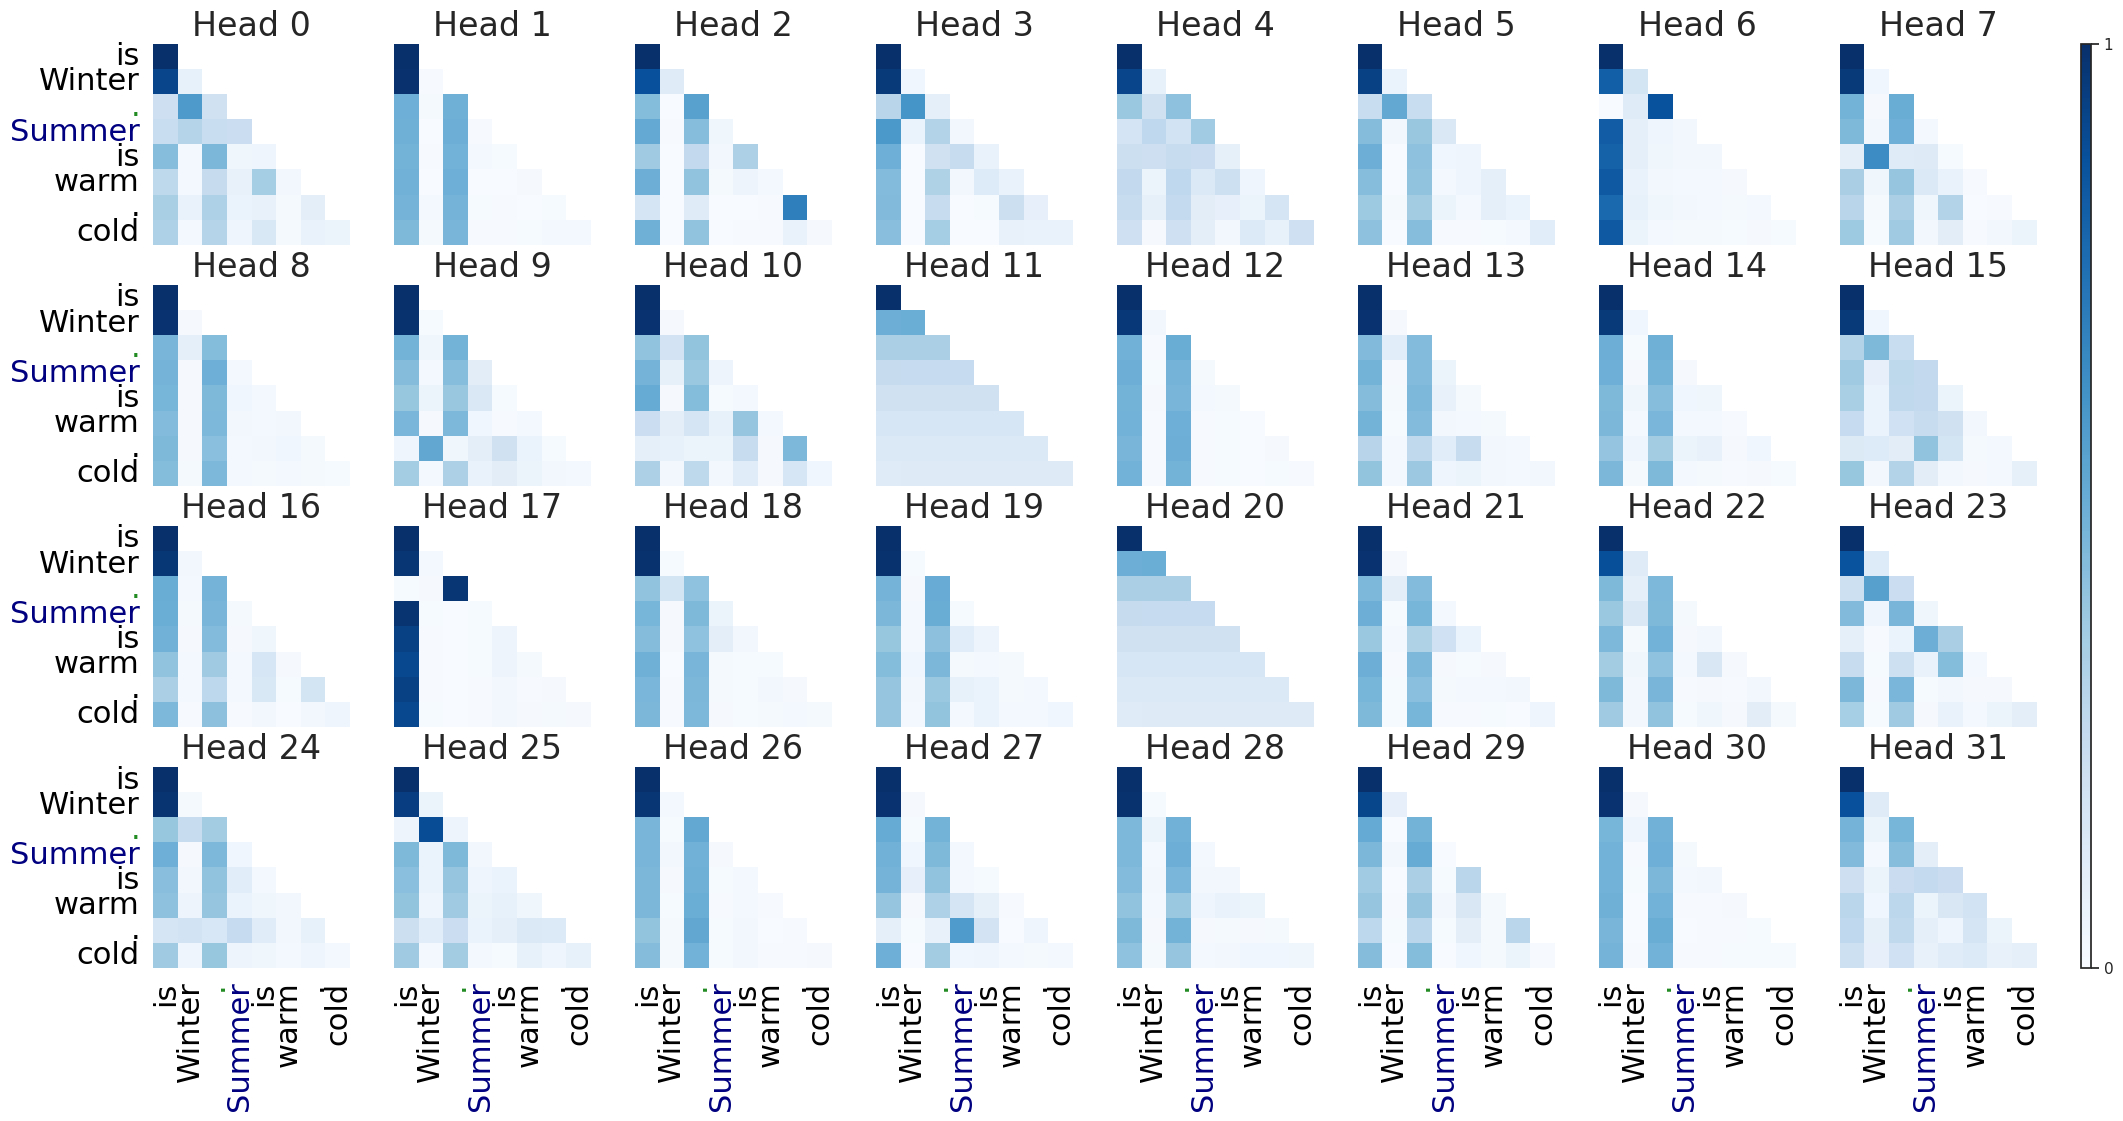
\includegraphics[width=\textwidth]{Figures/bos_study/attn_heads_shuffled.png}
    \caption{\small \textbf{Attention sinks with shuffled input in Layer 24 of OLMo.} In order to understand the impact of positional encodings when there is no \bos{} token, we shuffle the input of the test string ``Summer is warm. Winter is cold.'' in OLMo. We observe that there is still an attention sink on token \(0\), despite it being a random token that does not usually start sentences or phrases (since it is uncapitalized). This shows that the positional embedding, say via RoPE, has a large impact on the formation of attention sinks --- when the semantics of each token have switched positions, the attention sink still forms on the zeroth token.}
    \label{fig:bos_shuffle}
\end{figure}

Some models, such as OLMo, are not trained with a \bos{} token. Despite this, the first token of the input still frequently develops into a sink token. We can study the effect of positional encoding of the tokens on the attention sink phenomenon by shuffling the tokens before inputting them into the transformer, and observing how and why attention sinks form. If we do this with the phrase ``Summer is warm. Winter is cold.'' with OLMo, we observe that at Layer 24, there are many attention sink heads where the first token and first delimiter token share attention mass, even if the sentence is jumbled up and makes no grammatical sense. This points towards the observation that without a \bos{} token, the attention sink formation uses both positional data and, to a greater degree, the semantic data of each token. We leave studying this effect in greater detail to future work.


% \DP{Add ablation experiments with RoPE. It should work since that is the only place which has positional information.}


% \subsection{The attention logits on non-bos tokens decrease through the training dynamics}



